%!TEX root = ../../thesis.tex

\section{Radial velocity precision}
\label{section:rv_precision}
The first detections of extrasolar planets with the {RV} technique were hot-Jupiters; Jupiter mass planets in close orbits to their star.
The RV precision required to detect the first hot-Jupiter, 51 Peg b, was \todo{find mayor queloz precision achieved}~\cite{mayor_jupitermass_1995} \textbf{using }\todo{what reference} Since that time the instrumental development and the detection and observation techniques have been refined to achieve {RV} precisions better than 1\mps{}.
The recently commissioned ESPRESSO optical spectrograph is designed with the goal of achieving 10\cmps{}, which is the level of precision required to detect an Earth mass planet in an 1 year orbit round a Sun-like star.

Over the years the community has pushed the limits of this technique to smaller and smaller planetary masses.
An example is shown in \cref{fig:year_mass}.

\begin{figure}
    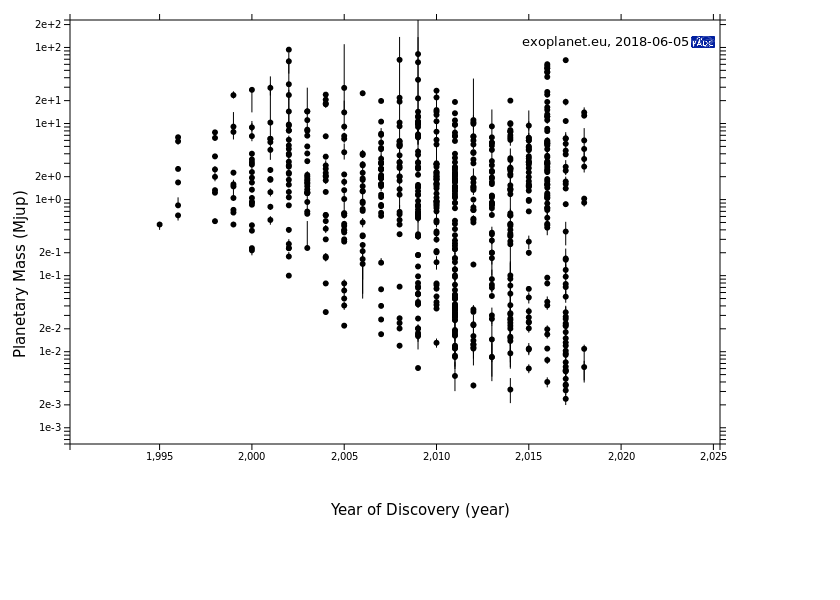
\includegraphics[width=0.8\linewidth]{figures/year_planet_mass.png}
    \caption{Mass of discovered planets verse year.
        From Exoplanet.eu}
    \label{fig:year_mass}
\end{figure}


{RV} amplitude scales with mass of the star \({M_{\star}}^{-2/3}\) and with the planetary orbital period \({P_{\textrm{orb}}}^{-2/3}\).

The detection of an Earth-mass planet inside the habitable zone around a solar-type star, the {RV} amplitude is 10\cmps{}.
If a planet with the same characteristics is instead orbiting an {M-dwarf}, the {RV} amplitude is larger than 1\mps{}.
This is due to two factors, the smaller mass of the host star, and the closer habitable zone, due to a lower luminosity output of the host.

\missingfigure{table of rv precisions}


\citet{artigau_optical_2018} recently compared archival spectra of Barnard's Star, an {M-dwarf}, and found that state-of-the-art atmosphere models over-predict the \emph{Y}- and \emph{J}-band {RV} content by more than a factor of \(\sim 2\), while under-predicting the \emph{H} and \emph{K}-band content by half.
{\red{} in this work we find similar?}

We are currently aiming to extend this work over the whole {M-dwarf} range, from {M0}-{M9}.

\todo{History of Precision calculations}
History of Precision calculations:
Connes 1\,985 -
Bouchy et al.
2001  - photon noise limit on rv measurements.
\cite{figueira_radial_2016} - focus on {M-dwarfs} parameter range to specify new instrumentation windows to focus.
Reiners 2017 -  {CARMENES} sample.
Some precision
Pedros school section other precision source \({r}^{1.5}\)


The 1.5 factor.....


\missingfigure{Bouchy 2001 inspired precision plot.}
\todo{Bouchy inspired precision plot}
